\documentclass{article}
\usepackage[utf8]{inputenc}
\usepackage{graphicx}
\usepackage{verbatim}
\usepackage{subfiles} 
\usepackage{fancyhdr}
\usepackage{hyperref}
\usepackage{natbib}


\title{DevOps, Software Evolution \& Software Maintenance Rapport}
\author{Group I - Mike\\\\
Repository: \url{https://github.com/SanderBuK/DevOpsMinitwit}
\\\\
Helle Friis (hefr@itu.dk)\\Sander Krogh (sank@itu.dk)\\Thomas Dal (thda@itu.dk)\\Jeppe Møller (jemm@itu.dk)}

\date{May 2021}

\pagestyle{fancy}
\fancyhf{}
\rhead{Group Mike - hefr, sand, thda \& jemm}
\lhead{DevOps Rapport}
\rfoot{Page \thepage}

\begin{document}
\maketitle
\newpage
\tableofcontents
\newpage

\section{Introduction}
This report is written in the course "DevOps, Software Evolution and Software Maintenance" 2021 at the IT-University of Copenhagen.
The main purpose of this project was to refactor a small version of Twitter named "ITU-MiniTwit" written in Python into another programming language. We have chosen to implement it in C\#. Next, we have used many different DevOps tools such as a CI/CD chain, logging and static code analysis. We will reflect on tools used, and discuss further findings.



\section{System's Perspective}
\subsection{Design the systems}
We use the Repository design pattern\footnote{(Kudchikar 2019)}. The pattern is commonly used together with Entity Framework, which we also use. The business logic is also split up between users and messages, isolating methods regarding each, making it simple to get an overview of the methods.
\\\\
Our MiniTwit application uses the MVC pattern. We use razor pages as our view, our repositories as our model, and one main controller for information passing from our model to our view.
\\\\
Our API is built with the REST framework in mind. This means exposing simple GET/POST endpoints, whose only purpose is to send the call to the appropriate repository class, which then handles the request, and returns the result.

\subsection{Architecture of the systems} 
The architecture of our system is a monolithic architecture\footnote{(Microsoft 2020)}, meaning it is entirely self-contained, and it is run together as one. Although it's a monolithic structure, the different functionalities of the system are split into different folders. The main functionalities being the backend, frontend and database manipulation functions. The result of having a monolithic architecture is that, monitoring and logging are also deployed in the stack, which can be seen in Figure 1.
\\\\
The database itself is hosted on an external server. This is so whenever we are rebuilding the main server, or if it happens to go down, the database remains consistent, even when applying load balancing. We then connect to the database server using its credentials in a connection-string, in the main system.

\newpage
\begin{figure}[h!]
\centering
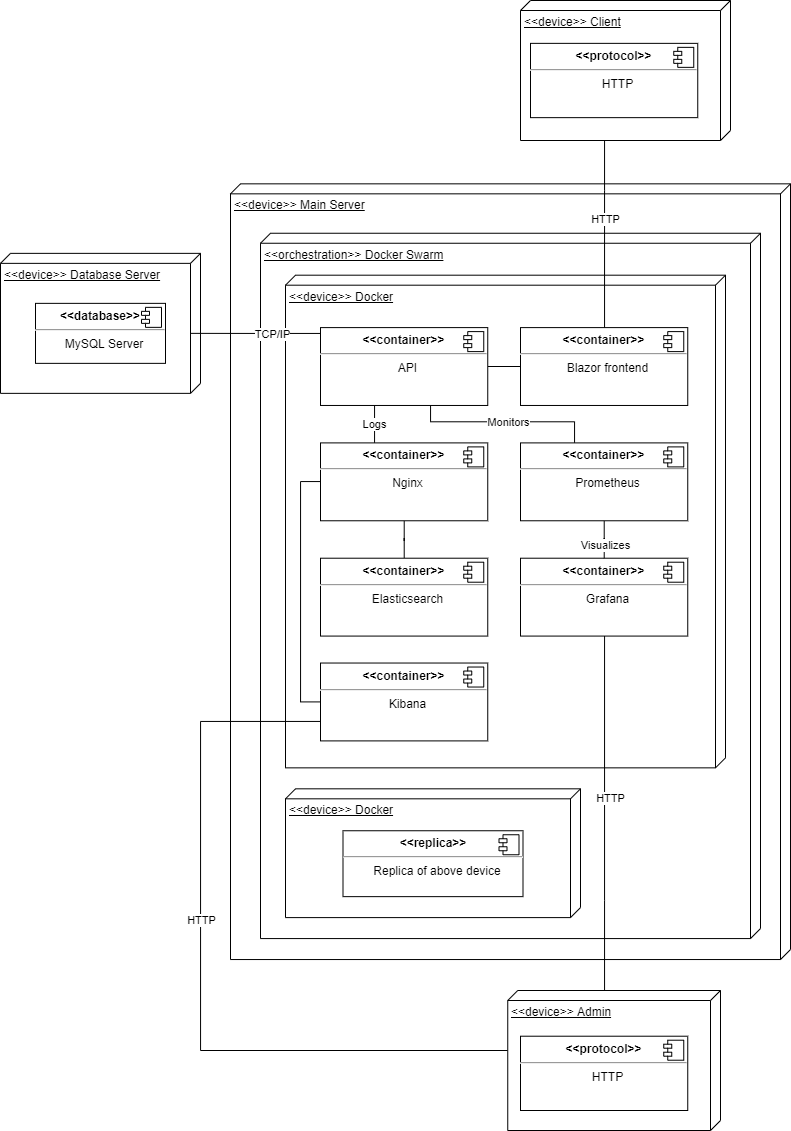
\includegraphics[width= \textwidth]{images/DeploymentDiagram.png}
\caption{Deployment diagram}
\end{figure}

\subsection{Dependencies}
This section serves to visualize the dependencies in our system, see Figure 2, and explain the usage of each of these.

\begin{itemize}
	\item \textbf{C\#\\}
	Our application uses several components of C\#. Firstly, Entity Framework Core. This allows for easy access to our MySQL database, and is the reason for using the repository design pattern. Secondly, we depend on ASP.Net Core, which includes a UI framework, namely Blazor. This is what our front-end is built in.
	\item \textbf{MySQL\\}
	MySQL is the database provider that we use. It contains all the data that we receive from the simulator.
	\item \textbf{Prometheus}\\
	This is our primary way of collecting metrics from our application. Prometheus supports both data pulling and pushing. We use data pulling, where we scrape certain monitoring-specific data, such as CPU-load and amount of requests to any endpoint, every 15 seconds from our application. The data is stored in a time series key-value pair.
	
 	\item \textbf{Grafana\\}
 	We use Grafana as a visualizer for data that we collect from Prometheus. Prometheus supports collecting data through PromQL queries, that lets us select and aggregate data. Grafana also allows for monitoring of MySQL databases, which we also visualize with graphs and counters.
 	
 	\item \textbf{Serilog}\\
 	Serilog creates logs for C\# projects. These can be formatted internally, and then sent to ElasticSearch
 	\item \textbf{Elasticsearch}\\
 	Used for searching logs, which are stored in dedicated log indexes.
 	\item \textbf{Kibana}\\
 	Kibana is the visualizer for the logs collected. It is used to filter and search through all logs provided by Elasticsearch.
 	
 	\item \textbf{Nginx\\}
 	Nginx is used for port forwarding, allowing the different Docker containers to communicate. This is mainly concerned with logging, having a communication channel with the API.
 	
 	\item \textbf{Vagrant}\\
 	Vagrant is used for starting or rebuilding our droplets. It has all of the specs and startup scripts that the droplet needs. The implementation of our CD pipeline made the use of vagrant files obsolete, unless a droplet would have to be replaced entirely.
 	
 	\item \textbf{Docker\\}
 	Docker is used for containerizing applications. Each component runs in a separate container. We use docker to create 'images' of our Blazor-app and the API. These images are pushed to DockerHub, which is then pulled to our application server. Each image is included in a Docker Compose file, which is used with Docker Swarm to deploy a complete stack at once. Each 'image' is then considered a 'service', which allows for horizontal scaling\footnote{(Lungu 2021)} of selected parts of the application. We swapped Vagrant for Docker Machine, as Docker Machine provisions a virtual machine in the same way that Vagrant does, but allows for better ease of use, using load balancing with Docker Swarm.
 	
 	\item \textbf{SonarCloud \& Better Code}\\
 	SonarCloud and Better Code are our main static code analysis tools. SonarCloud runs with our CI chain, on every push to the repository. With this you can add a limit as to how many warnings, and technical debt you will allow for each push. We haven't done so, but ideally should have. Better Code on the other hand is a website where you connect your repository, and can run analysis on it. We have done this, and added a badge to our README, to display our score.
 	\item \textbf{DigitalOcean}\\
 	We use DigitalOcean to provision droplet´s, which are virtual machines. This is where we host both our application and our database. It is possible to assign a 'floating IP' to a droplet, which ensures that if, for any reason, we had to swap any of existing droplets with a new one, we were able to use the same IP-address.
 	\item \textbf{GitHub Actions}\\
 	We use GitHub Actions for continuous deployment. It allows for several "steps", which could include testing when a push or pull request happens. We rely on GitHub Actions to push docker images to DockerHub and deploy these on our application server.
 	
\end{itemize}

\newpage
\begin{figure}[h!]
\centering
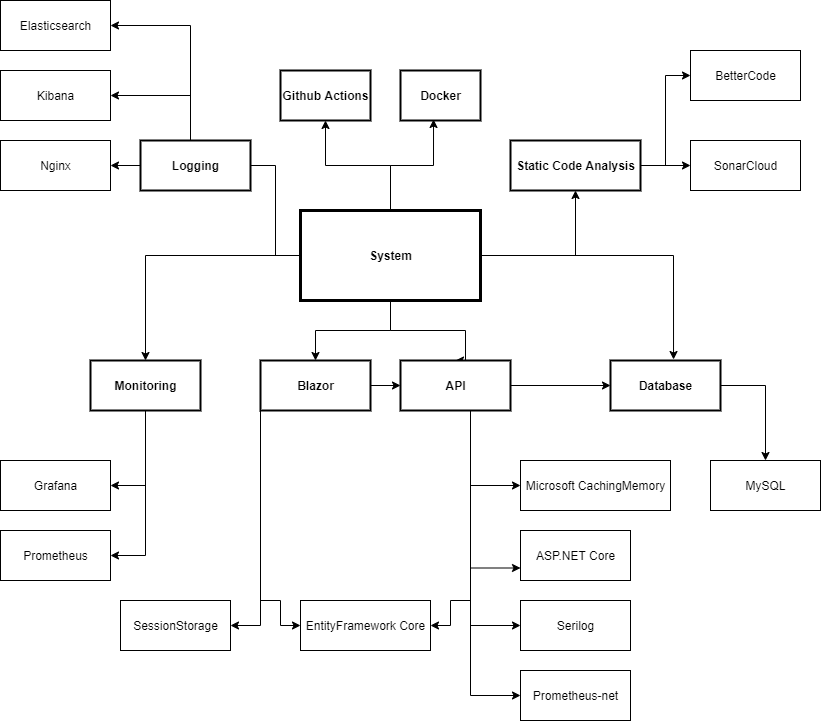
\includegraphics[width= \textwidth]{images/DependencyGraph.png}
\caption{Dependencies of the Minitwit system}
\end{figure}


\subsection{Important interactions of subsystems}
The data manipulation classes are dependant on a database, which in our case is a MySQL server running on an external droplet. The API and frontend are both dependant on the data manipulation methods, as they are used to request and add data to the database. The frontend uses the API controller directly, as opposed to accessing it through the endpoints. This is because they are deployed together, due to our system being a monolithic structure. Ideally it would use the APIs endpoints, but as it wasn't needed in our case, we decided not to.

\subsection{Current state of the system}
We have used different tools for static code analysis, but the ones giving us the most insightful results are SonarCloud, and BetterCode.
\\\\
According to BetterCode, our project fulfills all 10 out of 10 requirements, which includes code duplication and writing shor units of code, which can also be seen on the badge of our projects \verb|README.md| \footnote{https://github.com/SanderBuK/DevOpsMinitwit/blob/main/README.md}.
\begin{figure}[h]
    \centering
    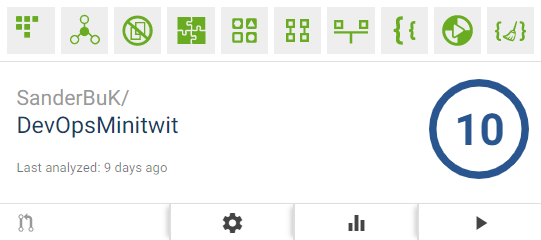
\includegraphics[width=0.7\textwidth]{images/bettercode.png}
    \caption{Status of our BetterCode analysis}
\end{figure}

SonarCloud on the other hand does highlight a few problems. This is mostly regarding commented out code, and unused fields. SonarCloud also shows some security hotspots, including visible connection-strings, which will be mentioned further in section 2.9.

\subsection{Licensing}
Grafana has a AGPL v3 license, which is a copyleft license. It imposes certain terms and conditions upon our system no matter which license we choose as a team. The open source policy of AGPL fits the philosophy of our team well enough, but imposing it on any derived work seems excessive. However, since Grafana is a very useful tool, we decided to also license our program under AGPL v3 to be able to use it. \footnote{https://github.com/SanderBuK/DevOpsMinitwit/blob/main/LICENSE}


\section{Process' perspective}

\subsection{Developer interactions}
Within the group we have created a Discord server, which has been our main form of communication. This has both been used for sharing documents, having meetings, and pair programming.
\\\\
Furthermore, we have used the "issues" feature on GitHub, using the provided Kanban board. This has also been used as a means of communication - communicating tasks to do, and how far along with the individual tasks, that we were.

\subsection{Team organization}
Our team consists of 4 developers, and we use the "Centralized Workflow"\footnote{(Pfeiffer 2021)}, where we have a mono-repository, which every developer synchronizes their work with. By the usage of "issues" on GitHub, work on the same modules or features by several developers at the same time is limited, as issues are moved to "In-progress" when a developer begins working on it. This serves to create transparency. The centralized workflow allows for us to have no power imbalances, and for each to provide value to the project evenly. We reduced our delaying steps \footnote{(Kim et al. 2016)} by everyone having the capabilities of code review and accepting pull request. In our team we have strived for a generative culture \footnote{ibid.}, meaning that we do not blame or reflect badly upon people making mistakes, but see it as part of the learning experience.

\subsection{Stages and tools included in the CI/CD chain}
Our CI/CD chain consists of a deployment stage, and multiple code analysis stages. These are all run through GitHub Actions, in our project repository.
\\\\
We have allocated a test step in our CI/CD chain, as automation of tests is very important for continuous deployment.
\\\\
The deployment stage consists of 2 steps, which are pushing and deploying. The first step builds the docker containers with a \verb|docker-compose| script\footnote{https://github.com/SanderBuK/DevOpsMinitwit/blob/main/docker-compose.yml}, and then pushes them up to \verb|DockerHub|. The next step then uses an SSH key to access our \verb|DigitalOcean| droplet containing our application, and runs a deployment script\footnote{https://github.com/SanderBuK/DevOpsMinitwit/blob/main/deploy.sh}, which pulls the images, and runs them.
\\\\
The deployment script is run on every push to our main branch, and not every release. This ensures that new features are directly deployed, after leaving development.

\subsection{Repository organization}
We are using a mono-repository where both the API and the Blazor-application is kept. This is to ensure that all modules that co-exist are versioned correctly, and will be able to run together, as an entity. This is very useful, as we have adopted GitHub Actions, where the API and Blazor is built from files from our repository, and pushed to Docker Hub. This simplifies the process of handling different versions of applications, and also simplifies the CI/CD chain, as only one repository is needed to collaborate and execute the program.

\subsection{Applied branching strategy}
We have been using a variant of the GitHub Flow\footnote{Pfeiffer 2021}. This involves creating an issue for every feature, fix or change needed to be done. Then creating a branch from "development" with a name along the lines of

\verb|feature/issue-num/descriptive-name|
\\
Then closing the issue when the branch is merged back into \verb|development|.
\newline \newline
When the code on \verb|development| has been tested and verified that it works, it can then be merged into main, triggering our CI/CD chain.

\subsection{Applied development process and tools supporting it}
We used the tools within GitHub a lot. For tasks we used GitHubs Issue feature. Furthermore we created labels, which allowed us to get a better overview of what was smaller bug fixes, and what was bigger features. We used GitHubs project board, in order to track what issues were open, closed, in progress, and in review.

\subsection{Monitoring}
For monitoring, we use Grafana and Prometheus. Prometheus has some standard metrics, which include average response times, total requests on each endpoints etc. We use some of these metrics, such as average response times, to tell if any of our end-points are creating a bottleneck. Furthermore, Grafana allows for monitoring of a MySQL connection. We added monitoring of our database-server, where we monitor total amount of users, messages \& follows. These are displayed in graphs, using Grafana, so it's easy to monitor the velocity of incoming requests, and helped us determine how much data we are receiving, and the speed of our endpoints.


\subsection{Logging}
Our logging logs all activity from the API, through Serilog. This includes all succeeding and failing API requests. This makes it able to search for failing endpoints, timeouts and other errors. 
\\\\
The logs that Serilog provide are sent directly to Elasticsearch, which we then visualize in Kibana. 

\subsection{Security assessment}
\subsubsection{Identifying assets}
We began the security assessment by identifying our assets
\begin{enumerate}
    \item \textbf{Database} - The database where our users' data is stored
    \item \textbf{Droplet} - both the application server and the database server
    \item \textbf{Public repository} - The MiniTwit repository that is publically available
\end{enumerate}

\subsubsection{Threat sources \& scenarios}
This is a description and elaboration of how our assets described in 3.9.1 may be accessed with malicious intent.
\begin{enumerate}
    \item An adversary gains access to any of the droplets and either alters them, or steals data. This could happen by eavesdropping or gaining physical access to any of our computers.
    \item An adversary gains hold of the credentials for the database, either eavesdropping, or altering our information. This could be done by finding the connection-string in the public repository.
    \item Someone gains access to DockerHub and pushes a new latest version of our application, which is then automatically pulled the next time we redeploy. This new version could hold malicious code.
    \item Someone reverse engineers the MD5 hashing algorithm, and may be able to decrypt the user passwords.
\end{enumerate}

\subsubsection{Risk analysis}
\begin{figure}[h!]
    \centering
    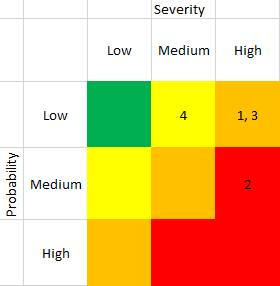
\includegraphics[width=0.7\textwidth]{images/risk-matrix.png}
    \caption{Risk analysis matrix. Y-axis is the likelyhood of each scenario happening. X-axis is the severity of any of the scenarios happening. Numbers 1-4 refer to the scenarios from 3.9.2}
\end{figure}
\subsubsection{Solution}
This section will discuss the solutions to the risk scenarios provided in 3.9.2
\begin{enumerate}
    \item Avoiding eavesdropping or limiting access to droplets - By defining users with different rights on our droplets, we would be able to limit access by IP-address to any of these users, disallowing any unauthorized IP-addresses to connect to our droplets. This would of course still leave us vulnerable to IP-spoofing
    \item Database credentials - This could be avoided by using environment variables on the droplet, or secrets in GitHub Actions. 
    \item DockerHub access or altering of images - This could be solved by only allowing commits from the team, thus disallowing alteration of the code from adversaries. Furthermore, DockerHub access could be limited by using secrets, thus limiting the possibility of pushing images to DockerHub 
    \item MD5 hashing algorithm - It is difficult to say that hashing algorithms will never be reverse-engineered. To make our passwords more secure, we would be able to use "salt" and "pepper"\footnote{(Lin 2016)}.
\end{enumerate}

\subsubsection{Pen-testing}
During our security assessment, we used both Nmap and WMAP. It yielded no obvious security flaws, but did show the container names of the application-server. It also showed that the OpenSSH was version 7.9, but according to www.cvedetails.com, there are no known vulnerabilities of this version. The result of the WMAP scan was that port 80 was open, which was quite obvious. It seemed that no security flaws were found using WMAP either.
\\\\
We made a mistake only scanning for vulnerabilities on the application server, as shortly before the simulator stopped, the database-server was hacked. This meant that all in-going data to the MySQL database was being intercepted, and dropped from our own tables. We found that we had not went through the MySQL Secure Installation \footnote{https://devanswers.co/install-secure-mysql-server-ubuntu-20-04/}, and had left a couple of vulnerabilities. Also, when creating the database, we allowed all IP-addresses to connect to the 'admin' user, which allowed for access to the MiniTwit tables. This, coupled with our connection string visible on a public repository, resulted in a very insecure database server. To solve this, we went through the secure installation, and only allowed for access to the MiniTwit table either through the root user, or from the floating IP-address that we had assigned our application-server.

\subsection{Applied strategy for scaling and load balancing.}
We tried our hands at using Docker-Swarm to scale and load balance our system. This involved creating docker-machines, to host our application.
\\\\
As the stack grew with things like logging, all of our droplet's RAM was utilized. This meant that the Kibana server wouldn't start, and we had problems with deploying our stack on the application server. We then decided to vertically scale our main server. For load balancing, we used Docker Swarm, in which we had our main server with the application itself, logging and monitoring. We then added a worker node with less CPU and RAM, where we scaled only our Blazor-application and our API. This ensured that we had a highly-available application.

\section{Lessons Learned Perspective}
\subsection{Evolution and refactoring}
We started off using an SQLite database file, as our database solution. This was not a good solution, since SQLite is in memory, and the main server would sometimes be down for redeployment or maintenance. Therefore we decided on an external server, with MySQL running. After migrating, it became a lot easier, but the process of extracting the data and moving it to a new server was very difficult and time consuming. Therefore, spending time deciding what technologies and solutions we used, would have saved a lot of time down the line.

\subsection{Operation}
As previously mentioned, our database was hacked, because we had our connection string visible in a public repository. Even though we were told it would be fine for this course, we definitely learned a lesson in security, that even though it sometimes feels unnecessary to take safety precautions, you should expect the worst.

\subsection{Maintenance}
We learned that when searching for tools, it is easy to find one that seems to fit, and get stuck on that one. Especially in this course where we are recommended tools. However sometimes the tools may not work as expected, or maybe doesn't fit your use case well. From that we have learned that it's important to research multiple tools, and weigh the pros and cons of all of them. There are multiple ways of implementing different technologies, and it can require some research to find a suitable solution.

\section{Conclusion}
In the course we have learned how to refactor an application to a modern language, updating its dependencies accordingly. Furthermore, we have learned about what choices you have to make in DevOps, including branching strategies, ways of organizing the team, etc. We have chosen the workflows we deemed the best fit for our use cases. We learned to use monitoring and logging to maintain our system, and decide what kind of scaling to apply in a given situation. Finally, we have learned how to maintain a system and use CI/CD to minimize downtime, while adding new functionality. 

\nocite{*}
\newpage
\bibliographystyle{plain}
\bibliography{bib}

\end{document}
